%%%%%%%%%%%%%%%%%%%%%%%%%%%%%%%%%%%%%%%%%%%%%%%%%%%%%%%%%%%%%%%%%%%%%
% LaTeX Template: Project Titlepage Modified (v 0.1) by rcx
%
% Original Source: http://www.howtotex.com
% Date: February 2014
% 
% This is a title page template which be used for articles & reports.
% 
% This is the modified version of the original Latex template from
% aforementioned website.
% 
%%%%%%%%%%%%%%%%%%%%%%%%%%%%%%%%%%%%%%%%%%%%%%%%%%%%%%%%%%%%%%%%%%%%%%

\documentclass[11pt]{report}
\usepackage[a4paper]{geometry}
\usepackage[myheadings]{fullpage}
\usepackage{fancyhdr}
\usepackage{lastpage}
\usepackage{graphicx, wrapfig, subcaption, setspace, booktabs}
\usepackage[T1]{fontenc}
\usepackage[font=small, labelfont=bf]{caption}
\usepackage{fourier}
\usepackage[protrusion=true, expansion=true]{microtype}
\usepackage[english]{babel}
\usepackage{sectsty}
\usepackage{url, lipsum}
\usepackage{amsmath}
\usepackage{pgfplots, pgfplotstable}
\usepackage{caption}


\newcommand{\HRule}[1]{\rule{\linewidth}{#1}}
\onehalfspacing
\setcounter{tocdepth}{5}
\setcounter{secnumdepth}{5}


%-------------------------------------------------------------------------------
% HEADER & FOOTER
%-------------------------------------------------------------------------------
\pagestyle{fancy}
\fancyhf{}
\setlength\headheight{15pt}
\fancyhead[L]{Terrence Ho}
\fancyhead[R]{Experiment 1}
\fancyfoot[R]{Page \thepage\ of \pageref{LastPage}}
%-------------------------------------------------------------------------------
% TITLE PAGE
%-------------------------------------------------------------------------------

\begin{document}

\title{ \normalsize \textsc{Physics 4AL}
        \\ [2.0cm]
        \HRule{0.5pt} \\
        \LARGE \textbf{\uppercase{Experiment 2: Measurement of g}}
        \HRule{2pt} \\ [0.5cm]
        \vspace*{2\baselineskip}}

\date{}

\author{
        Terrence Ho | ID: 804793446 \\ 
        Date of Lab: April 25th, 2017 \\
        Lab Section: Tuesday, 5 P.M.\\
        T.A.: David Bauer\\
        Lab Partners: Kai Crane}

\maketitle
\tableofcontents
\newpage

%-------------------------------------------------------------------------------
% Section title formatting
\sectionfont{\scshape}
%-------------------------------------------------------------------------------

%-------------------------------------------------------------------------------
% BODY
%-------------------------------------------------------------------------------
% \section*{Overview}
% \addcontentsline{toc}{section}{Overview}
% There were two parts to this experiment in order to find the value of \(g\).  

\section*{Plots}
\addcontentsline{toc}{section}{Plots/Graphs}
\pgfplotstableread{
X Y
0.455 10.02932997
0.540 10.03121116
0.630 10.07361673
0.270 10.32525633
0.740 10.05046127
}\datatable

\pgfplotstableread{
X Y
0.455 10.02932997
0.540 10.03121116
0.630 10.07361673
0.740 10.05046127
}\datatableTwo

\begin{figure}[h!]
\begin{tikzpicture}
    \begin{axis}[
        title={Distance Dropped vs Acceleration of \(g\)},
        xlabel={\textbf{Distance \(D\) between Second Photogate and Landing Pad
        (m)}},
        ylabel={\textbf{Acceleration of \(g\) (m/s$^2$)}},
        xmin=0, xmax=1,
        ymin=9.5, ymax=10.5,
        xtick={0,.2,.4,.6,.8,1},
        ytick={9.7, 9.9, 10.1, 10.3, 10.5},
        % width=\textwidth-\widthof{100}-0.1cm,
        % width=0.8\textwidth,
        ymajorgrids=true,
        grid style=dashed,
    ]
    \addplot[only marks, mark = *] table {\datatable};
    \addplot[thin, red] table[y={create col/linear
    regression={y=Y}}]{\datatable};
    \addlegendentry{%
    $\pgfmathprintnumber{\pgfplotstableregressiona} \cdot D
    \pgfmathprintnumber[print sign]{\pgfplotstableregressionb}$}
    \end{axis}
\end{tikzpicture}
\captionsetup{labelformat=empty}
\caption{\textbf{Figure 2.1  Graph of measured distance between second photogate and
impact sensor.} The dots on the graph depict acceleration \(g\) for heights .455 m, .54
m, .63 m, .27 m, and .72 m.  The best fit line for this equation has the line
\(g = -0.53D + 10.38\), where \(g\) is acceleration due to gravity and \(D\) is
height of fall.}
\end{figure}
For the ball drop experiment, 
I do not expect that \(g\) should depend on \(D\), because acceleration due to
gravity is constant everywhere on Earth.  Thus, the trendline fitting \(g\) vs
\(D\) should be completely horizontal.  However, \textbf{Figure 2.1} indicates that there
is a slight downward slope of -0.53\(D\), showing acceleration decreases with greater dropped
distance.  Due to the placement of the data points, I can see that the
datapoint at 0.27m has a much higher measured acceleration value of 10.31
m/s$^2$ compared to an average of 10.03 m/s$^2$ for the other data values.
Thus, we can eliminate this linear dependence if we choose to ignore the
acceleration at 0.27m as an outlier.  Without that data point, it is clear that
the resulting trendline will be much flatter, with a slight slope of 0.11\(D\).
We can see in \textbf{Figure 2.2} on the next page that without the acceleration 
for height 0.27m, the trendline for gravity is nearly flat and constant.

\setlength{\parindent}{5ex}
\textbf{Figure 2.3} on the next page shows four quadratic trendlines of position vs time of a
photocomb dropping through a photogate. Trial 3 was saved for a scientific plot
at the end. Accelerations and uncertanties of these trials are shown in 
\textbf{Table 2.3}.  The length of the comb was measured to be 30.5 cm, and we 
found length $\lambda$ of each hole segment by dividing the total length by the 
number of holes, which was 35. Because of this method of calculating $\lambda$, 
our calculations of \(g\) included both systematic and statistical 
uncertainties, which are explained later in \textbf{Table 2.3}. The height of which 
the photocomb was dropped from is 85 cm.

\begin{figure}[h!]
\begin{tikzpicture}
    \begin{axis}[
        title={Distance Dropped vs Acceleration of \(g\)},
        xlabel={\textbf{Distance \(D\) between Second Photogate and Landing Pad
        (m)}},
        ylabel={\textbf{Acceleration of \(g\) (m/s$^2$)}},
        xmin=0, xmax=1,
        ymin=9.5, ymax=10.5,
        xtick={0,.2,.4,.6,.8,1},
        ytick={9.7, 9.9, 10.1, 10.3, 10.5},
        % width=\textwidth-\widthof{100}-0.1cm,
        % width=0.8\textwidth,
        ymajorgrids=true,
        grid style=dashed,
    ]
    \addplot[only marks, mark = *] table {\datatableTwo};
    \addplot[thin, red] table[y={create col/linear
    regression={y=Y}}]{\datatableTwo};
    \addlegendentry{%
    $\pgfmathprintnumber{\pgfplotstableregressiona} \cdot D
    \pgfmathprintnumber[print sign]{\pgfplotstableregressionb}$}
    \end{axis}
\end{tikzpicture}
\captionsetup{labelformat=empty}
\caption{\textbf{Figure 2.2  Second graph of measured distance between second photogate and
impact sensor.} The dots on the graph depict acceleration \(g\) for heights .455 m, .54
m, .63 m, and .72 m.  We disregard the acceleration measured for height 0.27m.  
The best fit line for this equation has the line
\(g = 0.11D + 9.98\).}
\end{figure}

\begin{figure}[h!]
    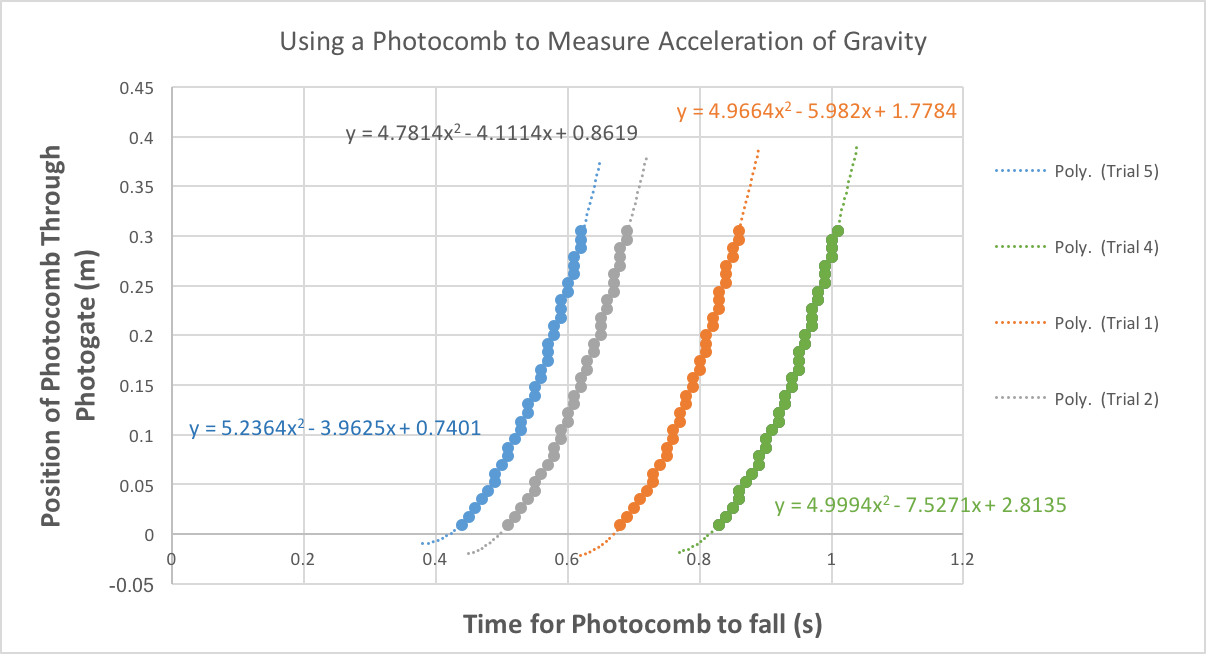
\includegraphics[width=\linewidth]{Photocomb1.png}
    \captionsetup{labelformat=empty}
    \caption{\textbf{Figure 2.3 Position of Photocomb through a photogate vs.
    time of fall.}} 
    Where t stands for time and d for distance fallen: 
    
    For Trial 1, d = (5.0 $\pm$ 0.4)t$^2$ -(5.9$\pm$ 0.6)t + (1.8 $\pm$ 0.2) in m.

    For Trial 2, d = (4.8 $\pm$ 0.4)t$^2$ -(4.1$\pm$ 0.4)t + (0.9 $\pm$ 0.1) in m. 

    For Trial 4, d = (5.0 $\pm$ 0.4)t$^2$ -(7.5$\pm$ 0.7)t + (2.8 $\pm$ 0.3) in m.

    For Trial 5, d = (5.2 $\pm$ 0.4)t$^2$ -(4.0$\pm$ 0.4)t + (0.7 $\pm$ 0.1) in m.

\end{figure}

\newpage
\section*{Derivation of Equation 2.1}
\addcontentsline{toc}{section}{Derivation of Equation 2.1}

Here we derive the equation used to calculate \(g\) for the ball drop
experiment. We first set the velocity \(V_1\) to be the distance \(d\) travelled between 
the first photogate and the second photogate over time \(T_1\).
Similiarly, the velocity \(V_2\) is equal to the distance \(D\) over time 
traveled \(T_2\) between the second photogate and the landing pad.

\[ V_1 = \frac{d}{T_1}   \qquad\text{and}\qquad     V_2 = \frac{D}{T_2} \]

We substitute these velocities into the kinetic equation \(V = V_o + g(t) \),
where \(V = V_2\), \(V_o = V_1\), and \(t\) is equal to the average of the two
times, or \(t = \frac{T_1 + T_2}{2} \).

\[ V_2 = V_1 + g\Bigg(\frac{T_1 + T_2}{2}\Bigg) \]

By substituting in the values for \(V_1\) and \(V_2\), we get an equation that
only contains the units that Equation 2.1 contained.

\[ \frac{D}{T_2} = \frac{d}{T_1} + g\Bigg(\frac{T_1 + T_2}{2}\Bigg) \]

By rearranging the equation so that g is isolated, we end up with Equation 2.1.

\[ g = \frac{2}{T_1 + T_2}\Bigg(\frac{D}{T_2} - \frac{d}{T_1}\Bigg) \textrm{ , in
terms of m/s$^2$}\]

\section*{Data Tables}
\addcontentsline{toc}{section}{Data Tables}
\subsection*{Ball Drop Tables}
Below are three tables, \textbf{Table 2.1} showing the measured acceleration and the
uncertainties from the ball drop.  \textbf{Table 2.2} shows the individual contributions
to the uncertainty made by both statistical and systematic uncertainty for the
ball drop. The uncertainties in \textbf{Table 2.1} were derived by adding together both the
systematic uncertainty and statistical uncertainty in table \textbf{Table 2.2}. 
\textbf{Table 2.3} shows the measured acceleration and uncertainties of \(g\) 
calculated from dropping a photocomb through a photogate.  

% \begin{table}[H]
\begin{center}
    \begin{tabular}{|c | c | c | c |}
    \hline
    Trial & Photogate Spacing \(d\)(cm) & Gap to impact Sensor \(D\)(cm) & Measured Acceleration \(g\)(m/s$^2$) \\
    \hline
    1 & 8.00 $\pm$ 0.05 & 45.50 $\pm$ 0.05 & 10.03 $\pm$ 0.02 \\
    \hline
    2 & 8.00 $\pm$ 0.05 & 54.00 $\pm$ 0.05 & 10.03 $\pm$ 0.03 \\
    \hline
    3 & 8.00 $\pm$ 0.05 & 63.00 $\pm$ 0.05 & 10.07 $\pm$ 0.03 \\
    \hline
    4 & 8.00 $\pm$ 0.05 & 27.00 $\pm$ 0.05 & 10.32 $\pm$ 0.01 \\
    \hline
    5 & 8.00 $\pm$ 0.05 & 72.00 $\pm$ 0.05 & 10.05 $\pm$ 0.03 \\
    \hline
    \end{tabular}
\end{center}
\captionof*{table}{\textbf{Table 2.1 Experiment Results and calculated acceleration
    values.} The average calculated value of the acceleration due to gravity \(g\) is
10.10 $\pm$ 0.02 m/s$^2$.  The systematic and statistical uncertainties are not
the same. The following Table 2.2 lists out the contributions to
uncertainty systematic and statistical uncertainty made.}

\subsection*{Systematic and Statistical Uncertainty for Ball Drop}
\begin{center}
    \begin{tabular}{| p{1cm} | p{2cm} | p{3cm} | p{4cm} | p{4cm} |}
        \hline
        Trial & Photogate Spacing \(d\)(cm) & Gap to impact sensor \(D\)(cm) & 
        Systematic Uncertainty in Measured Acceleration \(g\)(m/s$^2$) &
        Statistical Uncertainty in Measured Acceleration \(g\)(m/s$^2$) \\
        \hline
        1 & 8.00 $\pm$ 0.05 & 45.50 $\pm$ 0.05 & $\pm$ 0.02 & $\pm$ 0.003\\
        \hline
        2 & 8.00 $\pm$ 0.05 & 54.00 $\pm$ 0.05 & $\pm$ 0.02 & $\pm$ 0.01 \\
        \hline
        3 & 8.00 $\pm$ 0.05 & 63.00 $\pm$ 0.05 & $\pm$ 0.02 & $\pm$ 0.01 \\
        \hline
        4 & 8.00 $\pm$ 0.05 & 27.00 $\pm$ 0.05 & $\pm$ 0.01 & $\pm$ 0.003\\
        \hline
        5 & 8.00 $\pm$ 0.05 & 72.00 $\pm$ 0.05 & $\pm$ 0.02 & $\pm$ 0.01 \\
        \hline 
    \end{tabular}
\end{center}
\captionof*{table}{\textbf{Table 2.2 Uncertainty due to Statistical and
    Systematic Uncertainty} 
    Systematic uncertainty was calculated by calculating g on the upper and
    lower limits of the height's uncertainty.  Uncertainty due to measurement in distances \(d\) and \(D\) was 0.05 cm, or
0.0005 m, because milimeters are the smallest unit on a meter stick.  
The best values for T$_1$ and T$_2$ were used along with the upper and lower
limits of d and D to calculate g$_{min}$ and g$_{max}$.  We then subtracted the 
g$_{min}$ and g$_{max}$ and divided by two to get systematic \(\delta g\).

Statistical uncertainty was found using Excel's regression analysis.
}

Uncertainty was derived by adding together both the statistical and systematic
uncertainty. The uncertainty is dominated by statistical uncertainty, because
the the average systematic uncertainty is $\pm$ 0.0072 m/s$^2$, while the average
statistical uncertainty is $\pm$ 0.018 m/s$^2$, almost 2.5 times more
contribution.  Thus, statistical uncertainty dominates the uncertainty of the
calculated acceleration. However, because statistical uncertainty was not 10
times greater than systematic uncertainty, we could not eliminate one form of
uncertainty.
% \begin{center}
%     \begin{tabular}{| p{1cm} | p{2cm} | p{2cm} | p{3cm} |}
%         \hline
%         Trial & Photogate Spacing \(d\)(cm) & Gap to impact sensor \(D\)(cm) & 
%         Statistical Uncertainty in Measured Acceleration \(g\)(m/s$^2$) \\ 
%         \hline
%         1 & 8.00 $\pm$ 0.05 & 45.50 $\pm$ 0.05 & $\pm$ 0.003 \\ 
%         \hline
%         2 & 8.00 $\pm$ 0.05 & 54.00 $\pm$ 0.05 & $\pm$ 0.01 \\ 
%         \hline
%         3 & 8.00 $\pm$ 0.05 & 63.00 $\pm$ 0.05 & $\pm$ 0.01 \\
%         \hline
%         4 & 8.00 $\pm$ 0.05 & 27.00 $\pm$ 0.05 & $\pm$ 0.003 \\ 
%         \hline
%         5 & 8.00 $\pm$ 0.05 & 72.00 $\pm$ 0.05 & $\pm$ 0.01 \\ 
%         \hline 
%     \end{tabular}
% \end{center}
% \captionof*{table}{\textbf{Table 2.3 Uncertainty due to Statistical Uncertainty}
%     Using the standard deviation equaiton on STDEV on Excel, the uncertainties
% were calculated by dividing the standard deviations by the square root N number
% of data points.
% \[\delta g = \frac{1}{\sqrt{N}} * \sqrt{\frac{1}{N-1} * \sum\limits_{i=1}^{N} \big(x_i
% - \bar{x} \big)^2}\] } 

\subsection*{Photocomb Table}
\begin{center}
    \begin{tabular}{| c | c |}
        \hline
        Trial & Measured Acceleration (m/s$^2$) \\
        \hline
        1 & 9.9 $\pm$ 0.4 \\
        \hline
        2 & 9.56 $\pm$ 0.4 \\
        \hline
        3 & 9.2 $\pm$ 0.3 \\
        \hline
        4 & 10.0 $\pm$ 0.4 \\
        \hline
        5 & 10.5 $\pm$ 0.3 \\
        \hline
    \end{tabular}
\end{center}
\captionof*{table}{\textbf{Table 2.3 Acceleration Values From Photocomb Drop}
The photocomb was dropped from a height of 0.85 m, and the length of the comb was
measured to be 0.305 m. With 35 holes in the comb, each $\lambda$ was calculated
to be 0.0087 m, where $\lambda$ is the length of each hole in the photocomb.}

\setlength{\parindent}{5ex}
Because we calculated $\lambda$ by dividing by the length of the comb by the
number of holes in the comb, we had to take into account systematic uncertainty
in our calculations of \(g\).  The systematic values for
acceleration were calculated by taking the top and bottom of the range of
uncertainty for a measurement ruler (which was 0.0005 m), finding the values of
\(g\) and subtracting them, and dividing by two.  The statistical uncertanties 
were obtained by regression analysis on Excel.  

Because the systematic uncertainty values were much smaller than the statistical 
uncertainty values, only the statistical uncertainty affected the final outcome 
of the calculated \(g\), and so systematic uncertainty was excluded from the
final calculation. On average, the systematic uncertainty was $\pm$ 0.02 m/s$^2$,
whereas the average statistical uncertainty was $\pm$ 0.36 m/s$^2$, more than 10 times
greater. Systematic uncertanty had too few significant digits to be considered
in calculations.  The uncertainties of acceleration from the photocomb drop were
clealy dominated by statistical uncertainty.    

\section*{Conclusion}
\addcontentsline{toc}{section}{Conclusion}
The commonly accepted value of \(g\) is 9.80 m/s$^2$. The values of \(g\)
calculated in my ball drop experiment had low error $\%$ compared to the real
value regardless of the height, indicating that gravity is indeed constant and not
affect by the height with which an object was dropped from.  We can prove this
by calculating the difference between calculated and real values of
\(g\).  At .455 m, the percent of error was 2.3$\%$, at .54 m the error was 2.3$\%$, 
at .63 m the error was 2.8$\%$, at .27 m the error was 5.3$\%$, and at .72 m the 
error was 2.6$\%$.  

\setlength{\parindent}{5ex}
For the photocomb experiment, the error for Trial 1 was 1$\%$, the error for Trial 2 was
2.4$\%$, the error for Trial 3 was 6.1$\%$, the error for Trial 4 was 2$\%$, and
the error for Trial 5 was 7$\%$.  All the error percentages are low and indicate
our calculated values of \(g\) accurate relative to the true value of \(g\).
The average error percentage of the ball drop experiment was 3.06$\%$.  The
average error percentage for the photocomb experiment was 3.7$\%$.  

The most precise method of calculating the value of \(g\) was the ball drop,
which yielded more significant digits in the uncertainty calculations, which is
more precise (2 decimal places vs 1 decimal place).  
Based on average error percentage, we can see the ball 
drop experiment is more accurate in calculating the value of \(g\), because it
yields the closest value to true \(g\) on average.  However, it is interesting
to note that Trial 1 of the photocomb experiment resulted in the calculated value
that is closest to the real value of \(g\), with an error percentage of only 1$\%$. 
It could be said that the photocomb experiment is the most accurate way to get the closest
value of real \(g\), but this is not consistently replicable, so it cannot be said to
be the most accurate on average.  In fact, it also yielded the result with the greatest
error percentage at Trial 5(7$\%$), indicating its results are not entirely
reliable.  

For our uncertainty calculations, I went with the conservative route and added
together both the systematic and statistical uncertainties for the ball drop, 
because neither uncertianty value was 10 times smaller than the other.  This
process was chosen because there was no plausible reason to omit either and it
would increase the accuracy of our calculations. However, for the photocomb 
calculations, only the statistical uncertainties were used, because the 
systematic uncertainties were 10 times smaller than the statistical uncertainties.  

We notice that all the accelerations calculated from the ball drop were greater
than 9.8 m/s$^2$, and so we can conclude that when the experiment was being
conducted, the ball was given a slight push when it was dropped through the
photogates, explaining the higher than normal values for \(g\).  The next time
this experiment is conducted, we must make sure to not give the ball any
initial velocity when dropping the ball.

\section*{Report: Scientific Plots}
\addcontentsline{toc}{section}{Report}
\begin{figure}[h!]
    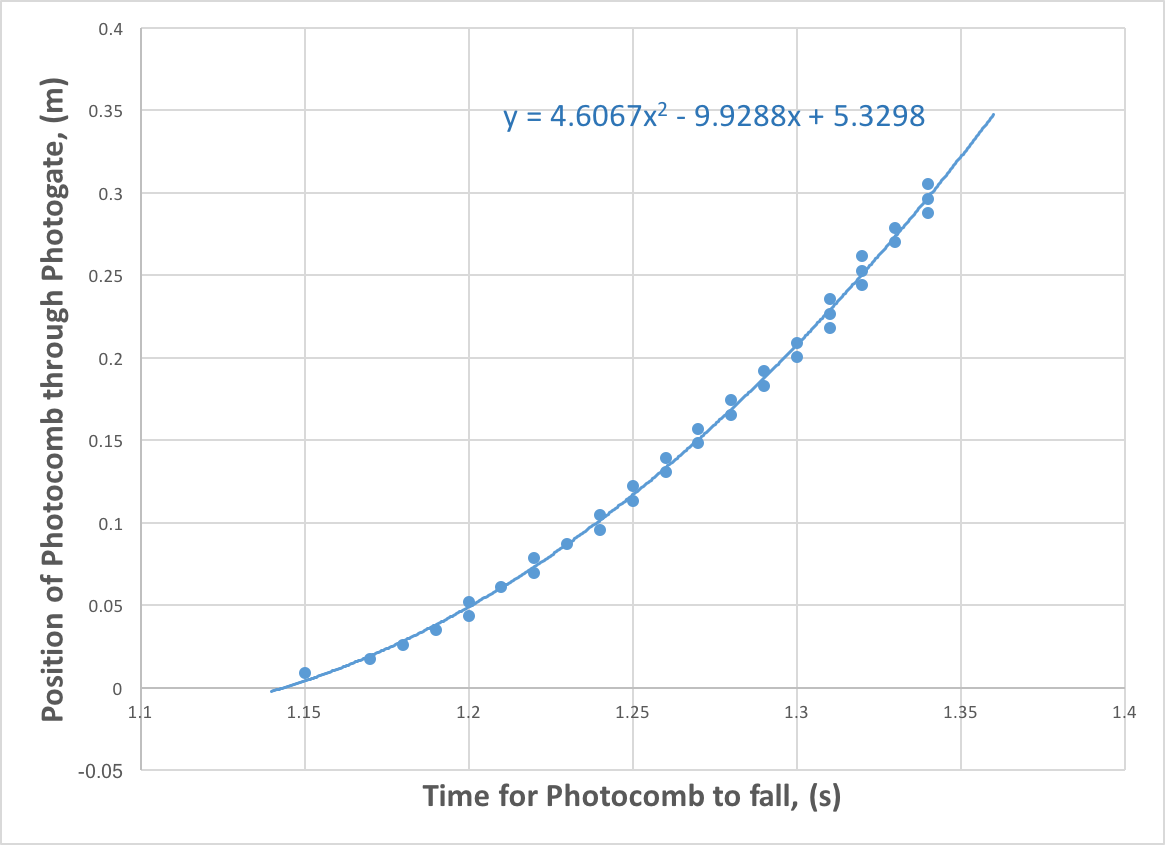
\includegraphics[width=\linewidth]{Photocomb2.png}
    \captionsetup{labelformat=empty}
    \caption{\textbf{Figure 2.4  Measuring value of acceleration by tracking the
    time a photocomb takes to fall through a photogate.}  The data is a fit line
    to the quadratic curve \(y = ax^2 + bx + c\), which shows that distance the 
    photocomb falls per second increases as time and that it is accelerating.  
    The fit line is \(y = (4.6 \pm 0.3)x^2 - (9.9 \pm 0.8)x + (5.3 \pm 0.5)\), 
    where y stands for distance fallen and x stands for time passed. The curves
of the graph have been extended slightly to show that the fit line is indeed a
parabola, which supports our decision to fit this data to a quadratic equation.}
\end{figure}

\textbf{Figure 2.4} above depicts the position of a photocomb dropped from
rest and accelerated by gravity over time.  By fitting the quadratic equation 
to our position vs time graph, we can find the value of the photocomb's 
acceleration due to gravity \(g\). Because the slope of the position vs time
graph is not constant but instead increasing, we determine that the photocomb is
speeding up and accelerating positively.  Because acceleration is position 
differentiated twice, we can see the value of \(g\) in this fit line is 
(9.8 $\pm$ 0.6)m/s$^2$, or twice the value of the constant before the x$^2$.  

The uncertainty of this calculated value comes wholly from statistical uncertainty. Systematic
uncertainty would stem from differences in measurements, and turned out to be 10
times smaller than statistical uncertainty.  The length of the photocomb used in
this experiment was measured to be 30.5 cm.  The uncertainty of the ruler was
0.05 cm, or half the smallest measurement unit, which was a millimeter.
Systematic uncertainty was calculated by taking the upper and lower bounds of
the measured length of the photocomb and finding \(g\) for those values,
subtracting \(g\)$_{max}$ and \(g\)$_{min}$ and dividing by two. Statistical
uncertainty was calculated using Excel's quadratic regression analysis.  
    
Our calculated value of \(g\) is very accurate.  The real value of
\(g\) is accepted to be 9.80 m/s$^2$, which matches our calculated value of
\(g\).  However, the precision of our calculation has a large range, from 
10.4 m/s$^2$ to 9.2 m/s$^2$.  Thus, our calculations are not precise.
Future improvements of this experiment would focus on increasing the precision
of the calculation and reducing the uncertainty range to less significant digits.  
This could be achieved by using machines that could track more precise
measurements and thus produce less statistical error, which accounts for most
uncertainty and error.

Word count: 303

%-------------------------------------------------------------------------------
% REFERENCES
%-------------------------------------------------------------------------------

% \addcontentsline{toc}{section}{References}

% Anand, U., 2010. The Elusive Free Radicals, \textit{The Clinical Chemist,} [e-journal] Available at:<\url{http://www.clinchem.org/content/56/10/1649.full.pdf}> [Accessed 2 November 2013]
% \newline
% \newline

% Biology Forums, 2012. \textit{Normal glomerulus. Acute glomerulonephritis.} [online] Available at: <\url{http://biology-forums.com/index.php?action=gallery;sa=view;id=9284}> [Accessed 23 October 2013].
% \newline
% \newline

% Budisavljevic, M., Hodge, L., Barber, K., Fulmer, J., Durazo-Arvizu, R., Self, S., Kuhlmann, M., Raymond, J. and Greene, E., 2003. Oxidative stress in the pathogenesis of experimental mesangial proliferative glomerulonephritis, \textit{American Journal of Physiology - Renal Physiology,} 285(6), pp. 1138-1148.
% \newline
% \newline

% Chien, C., Lee, P., Chen, C., Ma, M., Lai, M. and Hsu, S., 2001. De Novo Demonstration and Co-localization of Free-Radical Production and Apoptosis Formation in Rat Kidney Subjected to Ischemia/Reperfusion, \textit{Journal of the American Society of Nephrology,} 12(5), pp. 973-982.
% \newline
% \newline

% Couser, W., 1993. Pathogenesis of glomerulonephritis, \textit{Kidney International Supplements,} 42, pp. 19-26.
% \newline
% \newline

% De Gasparo, M., 2002. Angiotensin II and nitric oxide interaction, \textit{Heart Failure Reviews,} [e-journal] Available at:<\url{http://www.ncbi.nlm.nih.gov/pubmed/12379820}> [Accessed 26 October 2013]
% \newline
% \newline

% Edinburgh Renal Education Pages, 2012. \textit{Glomerulonephritis} [online] Available at: <\url{http://www.edrep.org/pages/textbook/glomerulonephritis.php}> [Accessed 25 October 2013].
% \newline
% \newline

% Forbes, J., Coughlan, M. and Cooper, M., 2008. Oxidative Stress as a Major Culprit in Kidney Disease in Diabetes, \textit{Diabetes,} 57(6), pp. 1446-1454.
% \newline
% \newline

% Geeky Medics, 2010. \textit{Glomerulonephritis} [online] Available at: <\url{http://geekymedics.com/2010/10/27/glomerulonephritis/}> [Accessed 25 October 2013].
% \newline
% \newline

% Gryglewski, R., Palmer, R., Moncada, S., 1986. Superoxide anion is involved in the break­down of endothelium derived relaxing factor, \textit{Nature,} 320, pp. 454-456.
% \newline
% \newline

% Halliwell, B., 2001. Free Radicals and other reactive species in Disease, \textit{Encyclopedia of Life Sciences,} [e-journal] Available at:<\url{http://web.sls.hw.ac.uk/teaching/level4/bcm1_2/reading/oxidative_stress/files/Oxidative_stress.pdf}> [Accessed 19 October 2013]
% \newline
% \newline

% Huang, H., Patel, P. and Salahudeen, A., 2001. Lazaroid compounds prevent early but not late stages of oxidant-induced cell injury: potential explanation for the lack of efficacy of lazaroids in clinical trials, \textit{Pharmacological Research,} 41(1), pp. 55-61.
% \newline
% \newline

% Klinger, J., Abman, S. and Gladwin, M., 2013. Nitric Oxide Deficiency and Endothelial Dysfunction in Pulmonary Arterial Hypertension, \textit{American Journal of Respiratory and Critical Care Medicine,} 188(6), pp. 639-646.
% \newline
% \newline

% Lindemann, I., Boettcher, J., Oertel, K., Pasternack, R., Heine, A. and Klebe, G. 2012. Inhibitors of Transglutaminase 2: A therapeutic option in celiac disease, \textit{To be Published,} [e-journal + PDB structure] Available at:<\url{http://www.ebi.ac.uk/pdbe-srv/view/entry/3s3s/summary}> [Accessed 24 October 2013]
% \newline
% \newline

% Mayo Clinic, 2011. \textit{Glomerulonephritis} [online] Available at: <\url{http://www.mayoclinic.com/health/glomerulonephritis/DS00503/}> [Accessed 20 October 2013].
% \newline
% \newline

% McCord, J., Roy, R. and Schaffer, S., 1985. Free radicals and myocardial ischemia. The role of xanthine oxidase, \textit{Advances in myocardiology,} [e-journal] Available at:<\url{http://www.ncbi.nlm.nih.gov/pubmed/2982206}> [Accessed 24 October 2013]
% \newline
% \newline

% National Health Service, 2012. \textit{Causes of glomerulonephritis} [online] Available at: <\url{http://www.nhs.uk/Conditions/Glomerulonephritis/Pages/Causes.aspx}> [Accessed 20 October 2013].
% \newline
% \newline

% Niaudet, P., 2013. \textit{Overview of the pathogenesis and causes of glomerulonephritis in children.} [online] Available at: <\url{http://www.uptodate.com/contents/overview-of- \ the-pathogenesis-and-causes-of-glomerulonephritis-in-children}> [Accessed 21 October 2013].
% \newline
% \newline

% Ronco, P., 2013. \textit{Mechanisms of glomerular crescent formation.} [online] Available at: <\url{http://www.uptodate.com/contents/mechanisms-of-glomerular-crescent-formation}> [Accessed 21 October 2013].
% \newline
% \newline

% Rutchik, J., 2013. \textit{Toxic Neuropathy Clinical Presentation.} [online] Available at: <\url{http://emedicine.medscape.com/article/1175276-clinical#a0216}> [Accessed 26 October 2013].
% \newline
% \newline

% R\&D Systems, 2013. \textit{Technical Information. Ischemia/Reperfusion Injury.} [online] Available at: <\url{http://www.rndsystems.com/cb_detail_objectname_SP96_Ischemia.aspx}> [Accessed 28 October 2013].
% \newline
% \newline

% Salahudeen, A., 1999. Free Radicals in Kidney Disease and Transplantation, \textit{Saudi Journal of Kidney Diseases and Transplantation,} 10(2), pp. 137-143.
% \newline
% \newline

% Sarma, A., Mallick, A. and Ghosh, A., 2010. Free Radicals and Their Role in Different Clinical Conditions: An Overview, \textit{International Journal of Pharma Sciences and Research,} 1(3), pp. 182-192.
% \newline
% \newline

% Shah, S., Baliga, R., Rajapurkar, M. and Fonseca, V., 2007. Oxidants in Chronic Kidney Disease, \textit{Journal of the American Society of Nephrology,} 18(1), pp. 16-28.
% \newline
% \newline

% The University of Utah, Unknown. \textit{Glomerulonephritis} [online] Available at: <\url{http://library.med.utah.edu/WebPath/RENAHTML/RENALIDX.html#8}> [Accessed 25 October 2013].
% \newline
% \newline

% Wang, C. and Salahudeen, A., 1994. Cyclosporine nephrotoxicity: attenuation by an antioxidant -inhibitor of lipid peroxidation in-vitro and in-vivo, \textit{Transplantation,} 58, pp. 940-946.
% \newline
% \newline

% Wang, C. and Salahudeen, A., 1995. Lipid peroxidation accompanies cyclosporine nephrotoxicity: effects of vitamin E, \textit{Kidney International,} 47, pp. 927-934.
% \newline
% \newline

% Weiss, S., 1989. Tissue Destruction by Neutrophils, \textit{New England Journal of Medicine,} 320, pp. 365-376.
% \newline
% \newline


\end{document}

%-------------------------------------------------------------------------------
% SNIPPETS
%-------------------------------------------------------------------------------

%\begin{figure}[!ht]
%    \centering
%    \includegraphics[width=0.8\textwidth]{file_name}
%    \caption{}
%    \centering
%    \label{label:file_name}
%\end{figure}

%\begin{figure}[!ht]
%    \centering
%    \includegraphics[width=0.8\textwidth]{graph}
%    \caption{Blood pressure ranges and associated level of hypertension (American Heart Association, 2013).}
%    \centering
%    \label{label:graph}
%\end{figure}

%\begin{wrapfigure}{r}{0.30\textwidth}
%    \vspace{-40pt}
%    \begin{center}
%        \includegraphics[width=0.29\textwidth]{file_name}
%    \end{center}
%    \vspace{-20pt}
%    \caption{}
%    \label{label:file_name}
%\end{wrapfigure}

%\begin{wrapfigure}{r}{0.45\textwidth}
%    \begin{center}
%        \includegraphics[width=0.29\textwidth]{manometer}
%    \end{center}
%    \caption{Aneroid sphygmomanometer with stethoscope (Medicalexpo, 2012).}
%    \label{label:manometer}
%\end{wrapfigure}

%\begin{table}[!ht]\footnotesize
%    \centering
%    \begin{tabular}{cccccc}
%    \toprule
%    \multicolumn{2}{c} {Pearson's correlation test} & \multicolumn{4}{c} {Independent t-test} \\
%    \midrule    
%    \multicolumn{2}{c} {Gender} & \multicolumn{2}{c} {Activity level} & \multicolumn{2}{c} {Gender} \\
%    \midrule
%    Males & Females & 1st level & 6th level & Males & Females \\
%    \midrule
%    \multicolumn{2}{c} {BMI vs. SP} & \multicolumn{2}{c} {Systolic pressure} & \multicolumn{2}{c} {Systolic Pressure} \\
%    \multicolumn{2}{c} {BMI vs. DP} & \multicolumn{2}{c} {Diastolic pressure} & \multicolumn{2}{c} {Diastolic pressure} \\
%    \multicolumn{2}{c} {BMI vs. MAP} & \multicolumn{2}{c} {MAP} & \multicolumn{2}{c} {MAP} \\
%    \multicolumn{2}{c} {W:H ratio vs. SP} & \multicolumn{2}{c} {BMI} & \multicolumn{2}{c} {BMI} \\
%    \multicolumn{2}{c} {W:H ratio vs. DP} & \multicolumn{2}{c} {W:H ratio} & \multicolumn{2}{c} {W:H ratio} \\
%    \multicolumn{2}{c} {W:H ratio vs. MAP} & \multicolumn{2}{c} {\% Body fat} & \multicolumn{2}{c} {\% Body fat} \\
%    \multicolumn{2}{c} {} & \multicolumn{2}{c} {Height} & \multicolumn{2}{c} {Height} \\
%    \multicolumn{2}{c} {} & \multicolumn{2}{c} {Weight} & \multicolumn{2}{c} {Weight} \\
%    \multicolumn{2}{c} {} & \multicolumn{2}{c} {Heart rate} & \multicolumn{2}{c} {Heart rate} \\
%    \bottomrule
%    \end{tabular}
%    \caption{Parameters that were analysed and related statistical test performed for current study. BMI - body mass index; SP - systolic pressure; DP - diastolic pressure; MAP - mean arterial pressure; W:H ratio - waist to hip ratio.}
%    \label{label:tests}
%\end{table}
